\clearpage
\paragraph{Soggetto 2}~

\vspace{1cm}

\noindent In questo paragrafo, vengono presentate le misure effettuate su un soggetto di sesso femminile, di 41 anni con carnagione chiara. Il soggetto si trovava in condizioni di riposo.

\vspace{0.5cm}

\noindent Di seguito sono riportate le acquisizioni effettuate utilizzando il sensore \textbf{MAX86916} su una finestra temporale di 10 secondi, in più siti di misura.

\subparagraph{Polpastrello indice sinistro}
Dalle acquisizioni riportate in figura \ref{fig:soggetto2_MAX86916_polpastrello}, effettuate sul polpastrello dell'indice della mano sinistra, si può notare come il segnale ottenuto sia di ottima qualità per tutte e quattro le lunghezze d'onda impiegate, confermando i risultati ottenuti con il soggetto 1, e anche le considerazioni fatte a livello teorico nel capitolo \ref{cap:sitimisura}. Infatti, dalle immagini riportate si possono distinguere chiaramente sia i picchi sistolici, sia diastolici e le tacche dicrotiche. Il segnale con ampiezza maggiore è quello del LED verde mentre i LED rosso e infrasso presentano l'ampiezza minore. Anche qui si possono individuare 10 picchi del segnale, stimando una frequenza cardiaca di 60 battiti al minuto.
\begin{figure}[h]
	\centering
	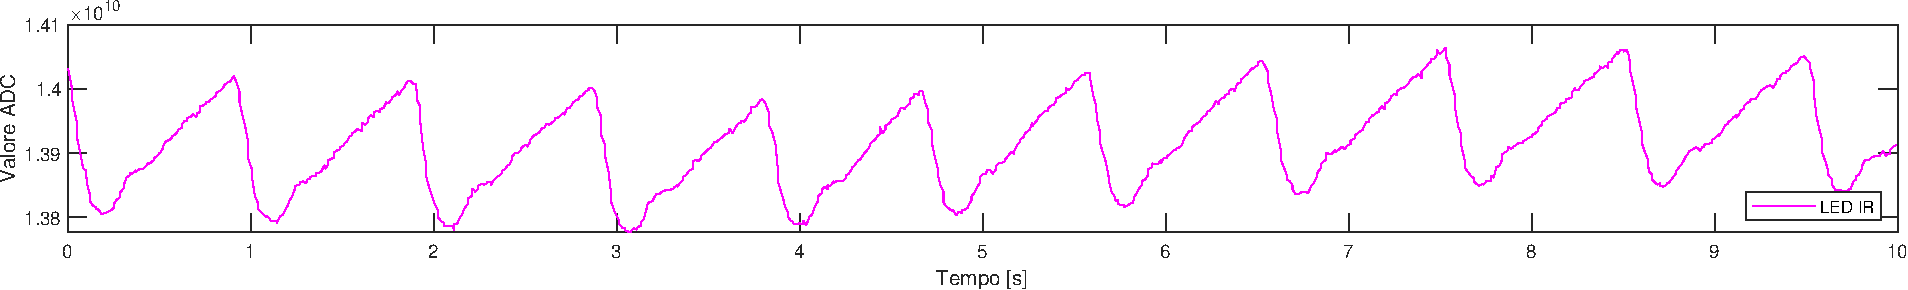
\includegraphics[width=1\linewidth]{ImageFiles/Misure Preliminari/Soggetto 2/max86916/polpastrello_ired}
	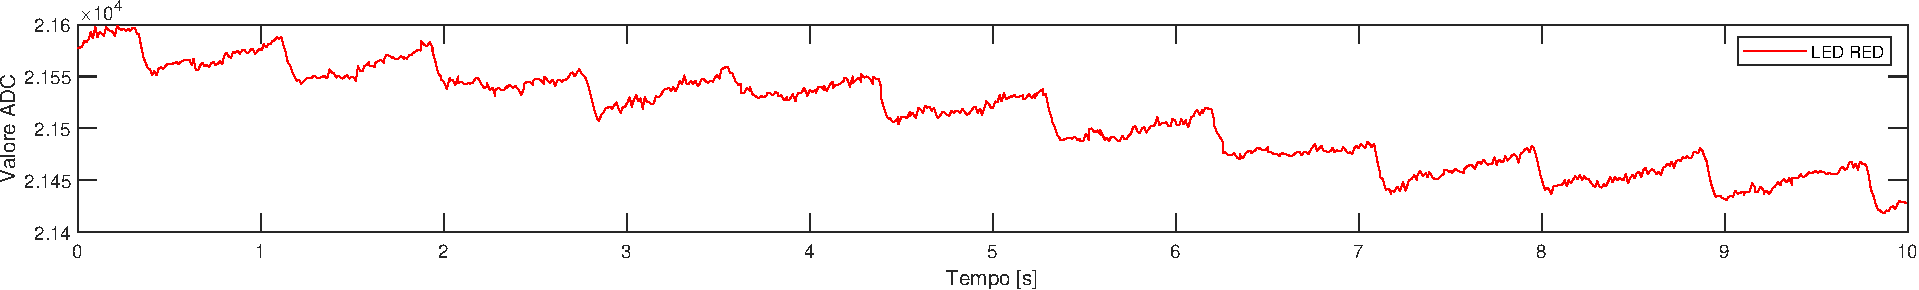
\includegraphics[width=1\linewidth]{ImageFiles/Misure Preliminari/Soggetto 2/max86916/polpastrello_red}
	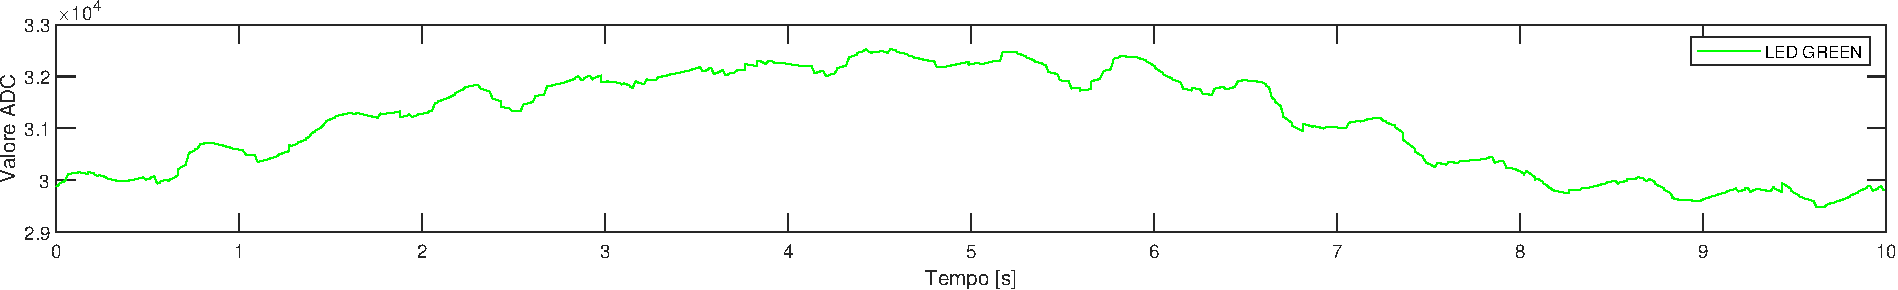
\includegraphics[width=1\linewidth]{ImageFiles/Misure Preliminari/Soggetto 2/max86916/polpastrello_green}
	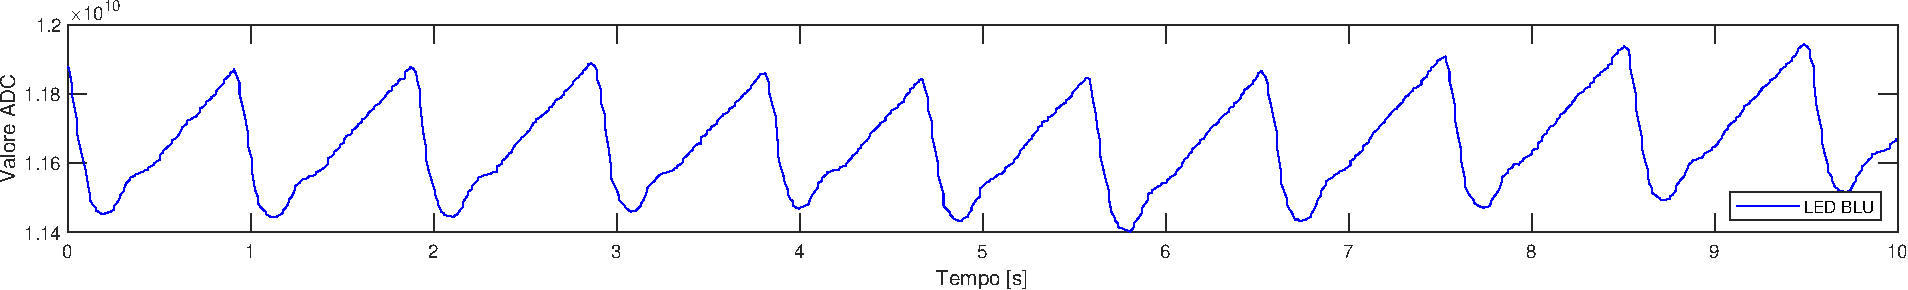
\includegraphics[width=1\linewidth]{ImageFiles/Misure Preliminari/Soggetto 2/max86916/polpastrello_blu}
	\caption{Soggetto 2 - Segnali PPG acquisiti sul polpastrello del dito indice sinistro con il sensore MAX86916.}
	\label{fig:soggetto2_MAX86916_polpastrello}
\end{figure}

\clearpage

\paragraph{Lobo orecchio destro}
Le acquisizioni ottenute sul lobo dell'orecchio destro presentano un segnale di qualità leggermente inferiore rispetto al sito precedente. Ciò è dovuto principalmente alla difficoltà della misura in questo sito. Tuttavia, la morfologia del segnale è evidente. Infatti, in figura \ref{fig:soggetto2_MAX86916_lobo}, si possono ancora apprezzare i picchi sistolici e diastolici su tutte le lunghezze d'onda impiegate. Il LED verde offre il segnale ad ampiezza maggiore. I picchi individuati sono 10, stimando una frequenza cardiaca di 60 battiti al minuto, coerente con il risultato ottenuto con le misure sul polpastrello.
\begin{figure}[h]
	\centering
	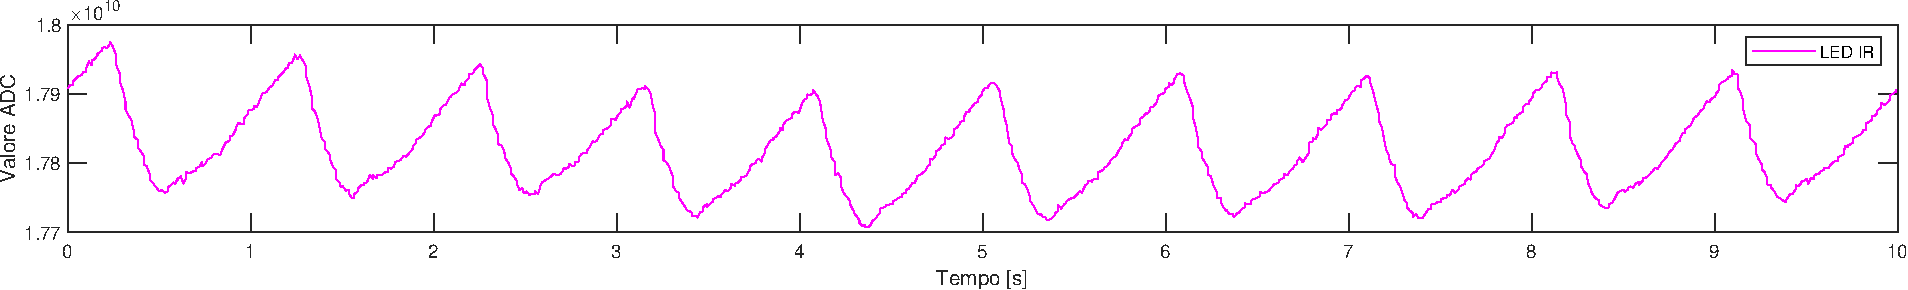
\includegraphics[width=1\linewidth]{ImageFiles/Misure Preliminari/Soggetto 2/max86916/lobo_ired}
	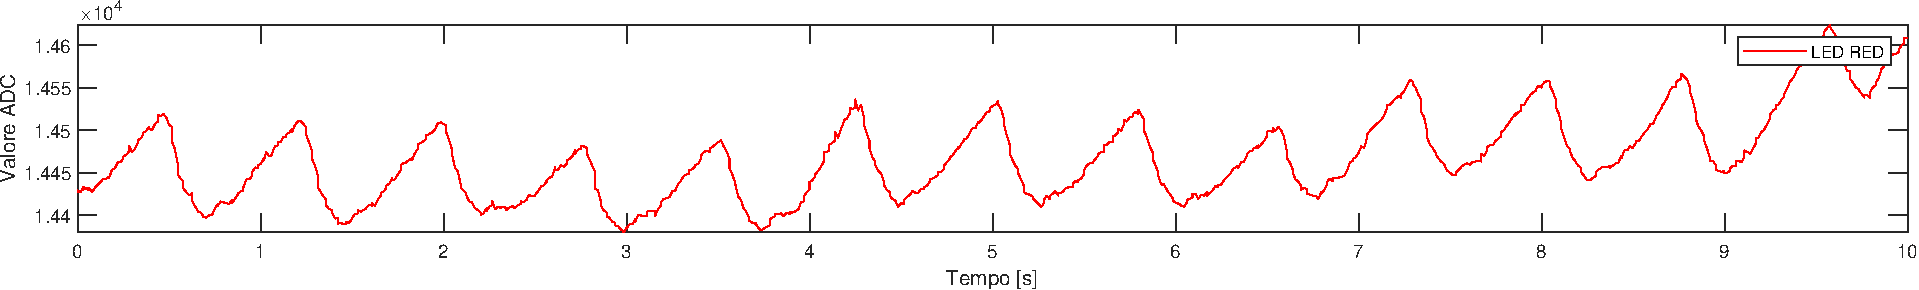
\includegraphics[width=1\linewidth]{ImageFiles/Misure Preliminari/Soggetto 2/max86916/lobo_red}
	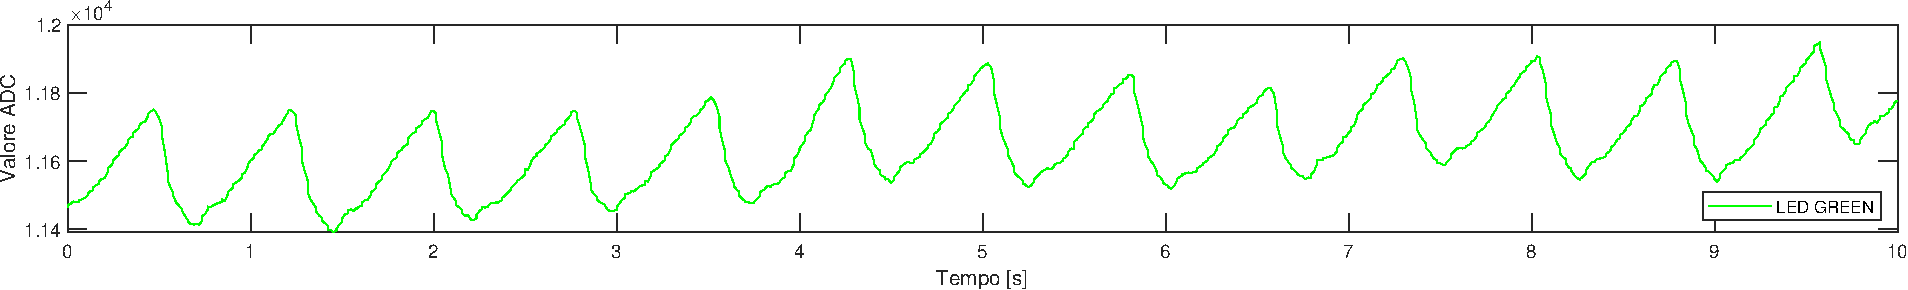
\includegraphics[width=1\linewidth]{ImageFiles/Misure Preliminari/Soggetto 2/max86916/lobo_green}
	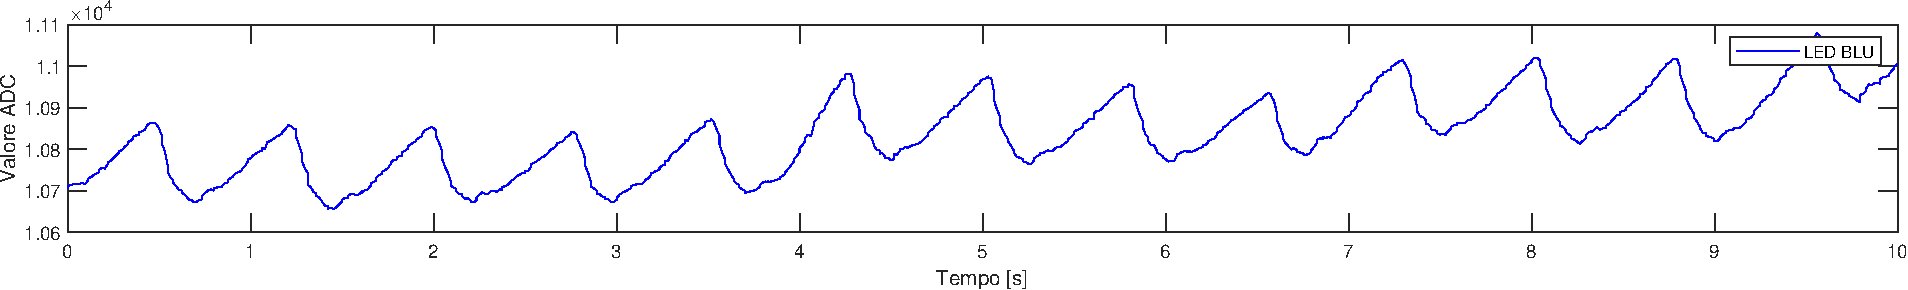
\includegraphics[width=1\linewidth]{ImageFiles/Misure Preliminari/Soggetto 2/max86916/lobo_blu}
	\caption{Soggetto 2 - Segnali PPG acquisiti sul lobo dell'orecchio destro con il sensore MAX86916.}
	\label{fig:soggetto2_MAX86916_lobo}
\end{figure}

\clearpage

\subparagraph{Polso antero-interno}

Le misure effettuate sulla zona del polso antero-interna sono più soggette a disturbi, principalmente dovuti a movimenti di natura involontaria. Come si può vedere in figura \ref{fig:soggetto2_MAX86916_polso}, questi disturbi sono più visibili per la luce rossa e infrarossa, mentre per la luce blu e verde il segnale si dimostra ancora pulito e chiaro. Nonostante ciò la qualità si può reputare buona, infatti sono ancora individuabili i picchi di interesse. Anche in questa misura il segnale ad ampiezza maggiore è quello del LED verde. La frequenza cardiaca stimata da questa acquisizione è di 60 battiti al minuto.
\begin{figure}[h]
	\centering
	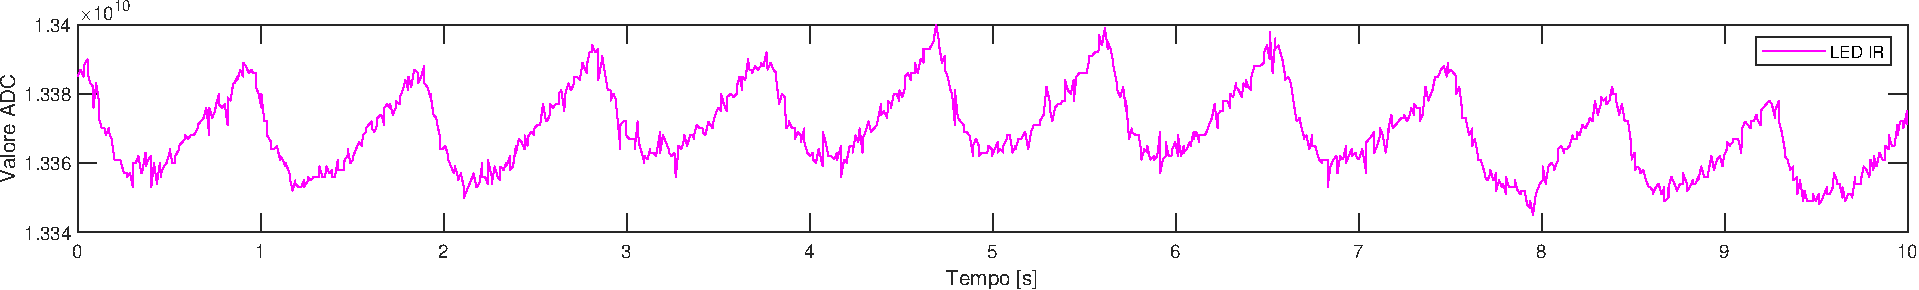
\includegraphics[width=1\linewidth]{ImageFiles/Misure Preliminari/Soggetto 2/max86916/polso_inferiore_ired}
	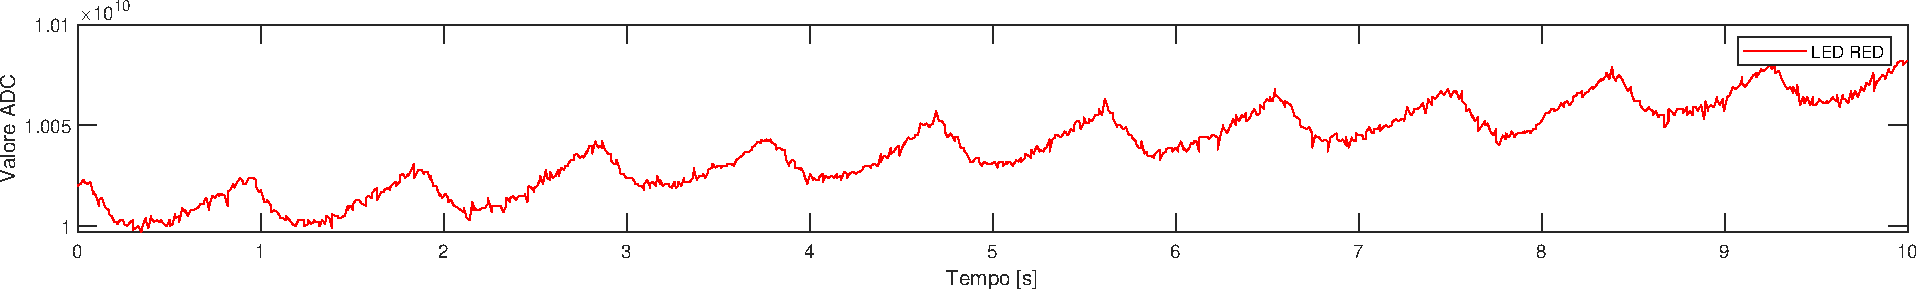
\includegraphics[width=1\linewidth]{ImageFiles/Misure Preliminari/Soggetto 2/max86916/polso_inferiore_red}
	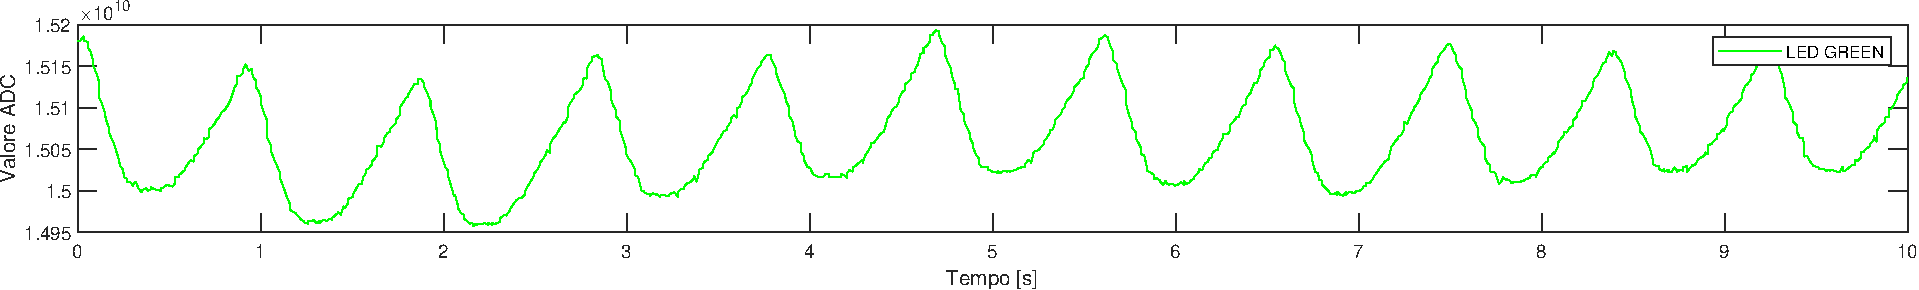
\includegraphics[width=1\linewidth]{ImageFiles/Misure Preliminari/Soggetto 2/max86916/polso_inferiore_green}
	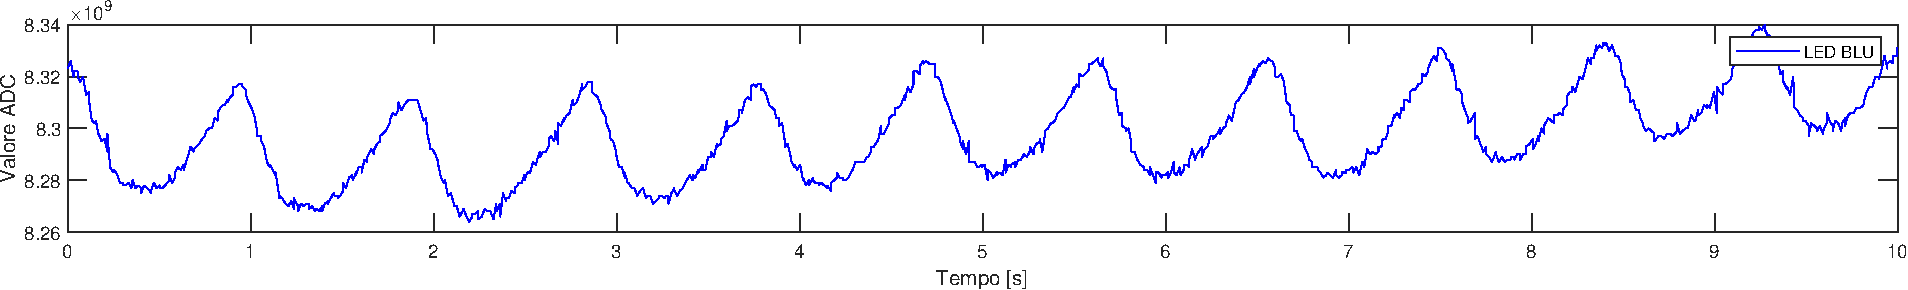
\includegraphics[width=1\linewidth]{ImageFiles/Misure Preliminari/Soggetto 2/max86916/polso_inferiore_blu}
	\caption{Soggetto 2 - Segnali PPG acquisiti sul polso destro con il sensore MAX86916.}
	\label{fig:soggetto2_MAX86916_polso}
\end{figure}

\clearpage

\subparagraph{Fronte}
Infine, in figura \ref{fig:soggetto2_MAX86916_fronte}, vengono riportati i risultati delle acquisizioni effettuate sulla fronte. I segnali ottenuti presentano una buona qualità. Osservando la componente AC dei segnali, il verde presenta un'ampiezza maggiore. Anche in questo caso si vede che la luce blu permette di identificare correttamente i picchi sistolici. Le misure risultano essere meno rumorose rispetto a quelle acquisite sul polso. La frequenza cardiaca stimata è di 60 battiti al minuto, confermando i precedenti risultati.

\begin{figure}[h]
	\centering
	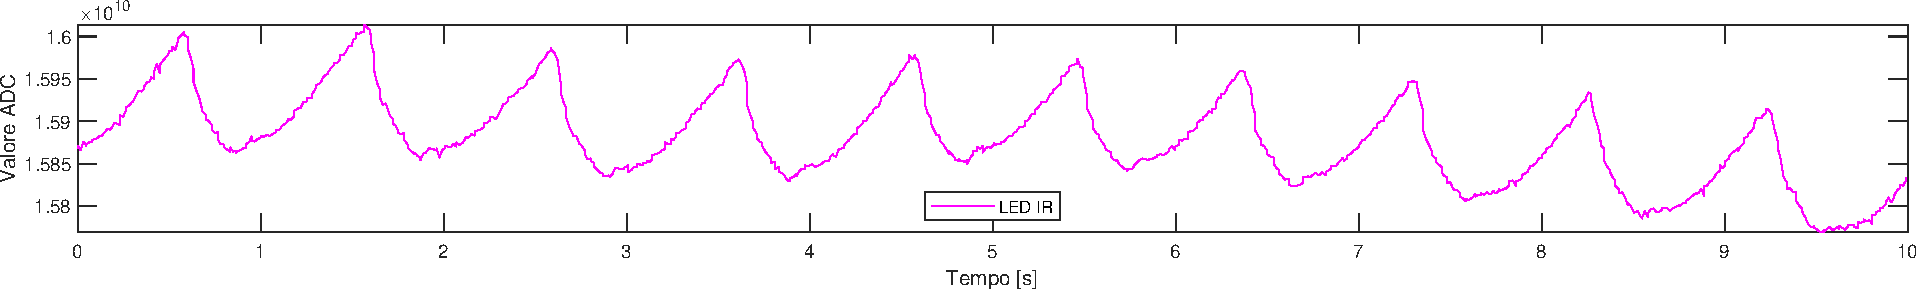
\includegraphics[width=1\linewidth]{ImageFiles/Misure Preliminari/Soggetto 2/max86916/fronte_ired}
	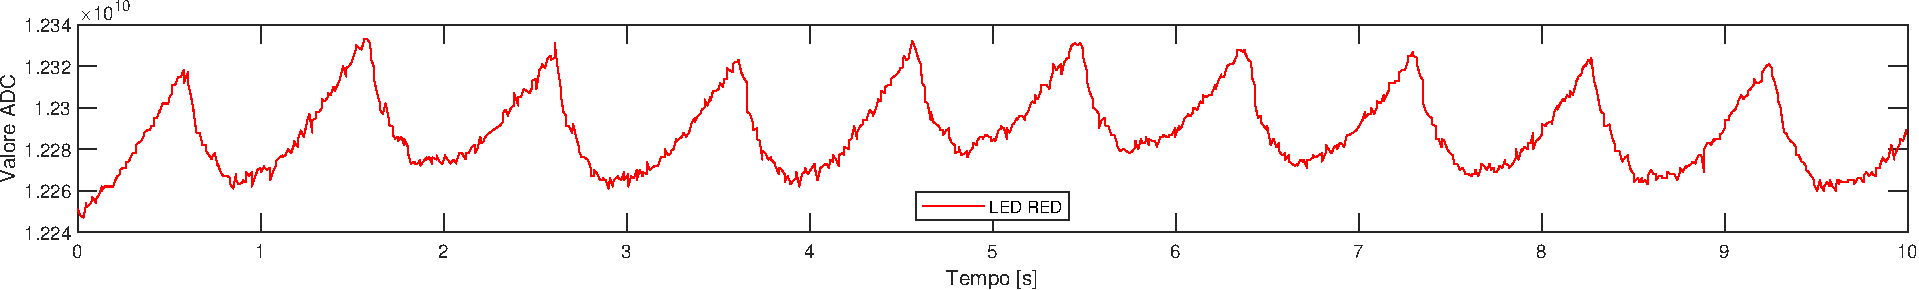
\includegraphics[width=1\linewidth]{ImageFiles/Misure Preliminari/Soggetto 2/max86916/fronte_red}
	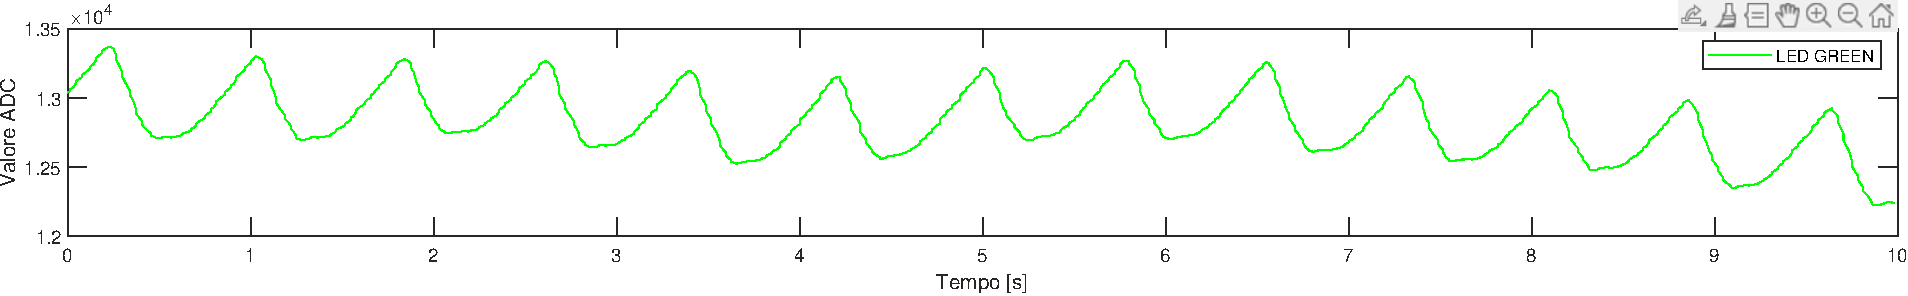
\includegraphics[width=1\linewidth]{ImageFiles/Misure Preliminari/Soggetto 2/max86916/fronte_green}
	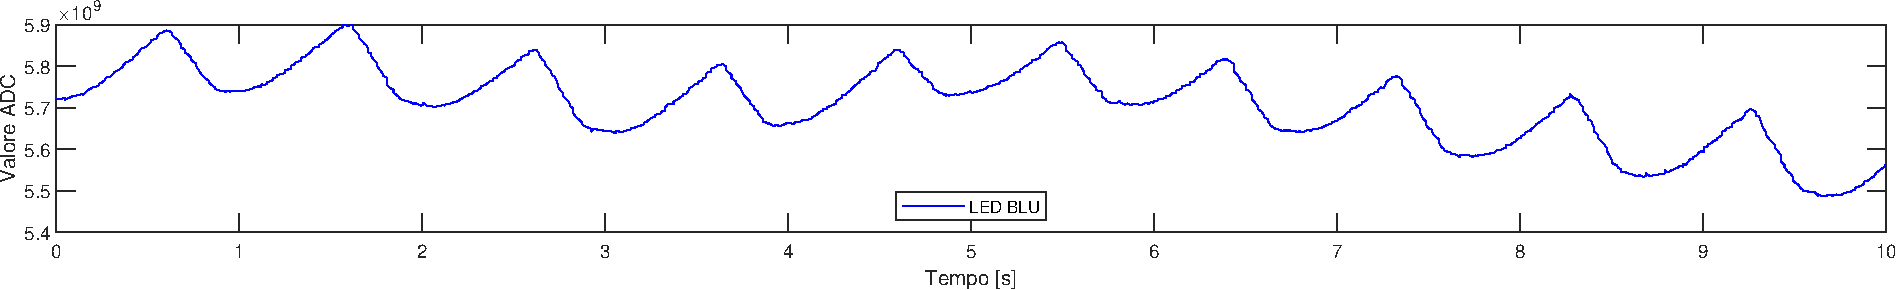
\includegraphics[width=1\linewidth]{ImageFiles/Misure Preliminari/Soggetto 2/max86916/fronte_blu}
	\caption{Soggetto 2 - Segnali PPG acquisiti sulla fronte con il sensore MAX86916.}
	\label{fig:soggetto2_MAX86916_fronte}
\end{figure}

\clearpage

Di seguito sono riportate le acquisizioni effettuate utilizzando il sensore \textbf{MAXM86161} su una finestra temporale di 10 secondi. Le acquisizioni ottenute sono state elaborate con un filtro a media mobile.

\subparagraph{Polpastrello indice sinistro}
Il segnale PPG ottenuto sul polpastrello del dito indice sinistro risulta essere di buona qualità e il tracciato del LED verde risulta avere l'ampiezza massima \Fig~\ref{fig:soggetto2_MAXM86161_polpastrello}. Questo risultato era prevedibile dal momento che il polpastrello è noto essere un ottimo sito di misura, come verificato sulle acquisizioni precedenti. Il filtro è stato applicato con una finestra di 10 campioni per il LED verde, di 20 per il LED rosso e 25 per quello infrarosso. I picchi del segnale sono 13, quindi la frequenza cardiaca stimata è di 78 battiti al minuto.

\begin{figure}[h]
	\centering
	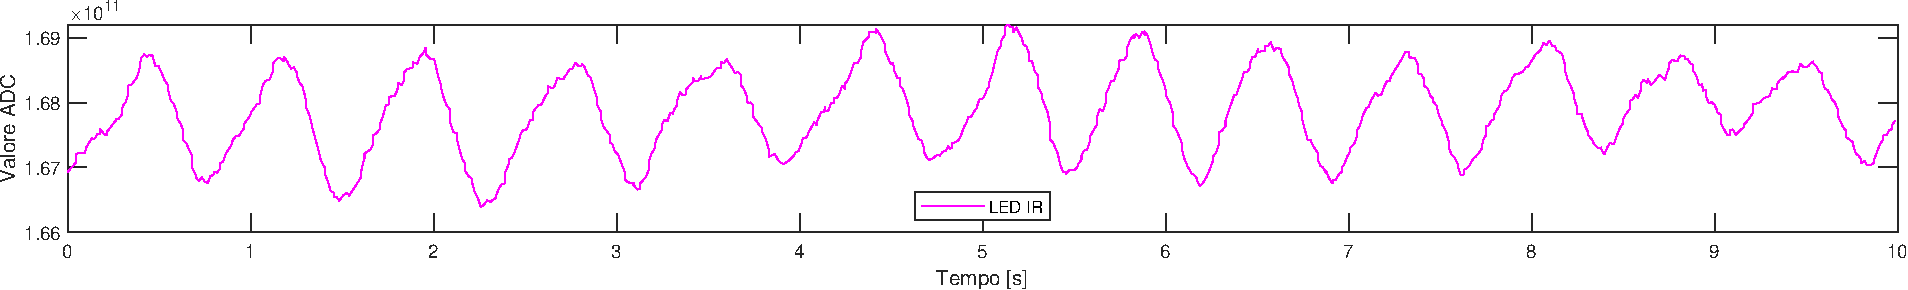
\includegraphics[width=1\linewidth]{ImageFiles/Misure Preliminari/Soggetto 2/maxm86161/polpastrello_ir_moving_avg}
	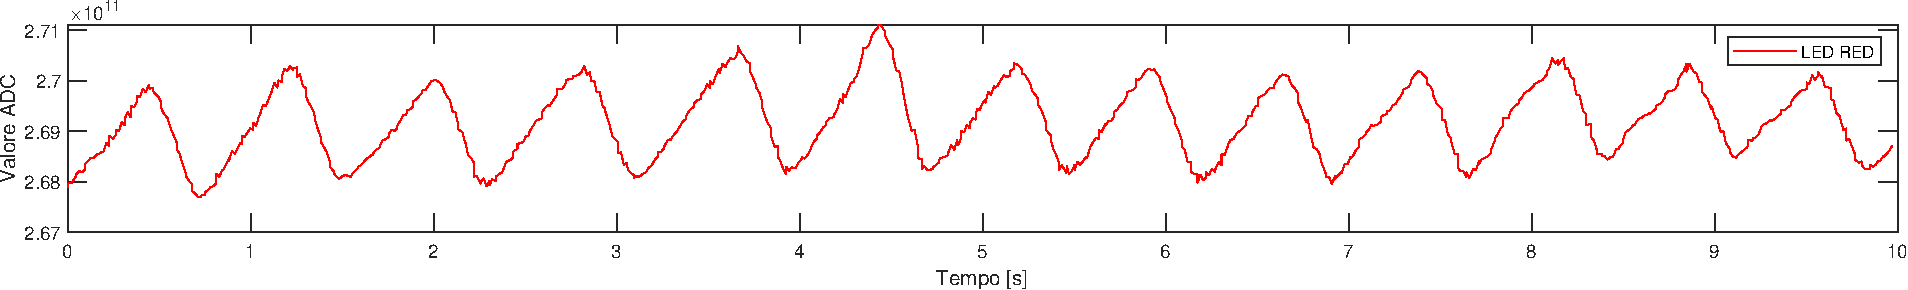
\includegraphics[width=1\linewidth]{ImageFiles/Misure Preliminari/Soggetto 2/maxm86161/polpastrello_red_moving_avg}
	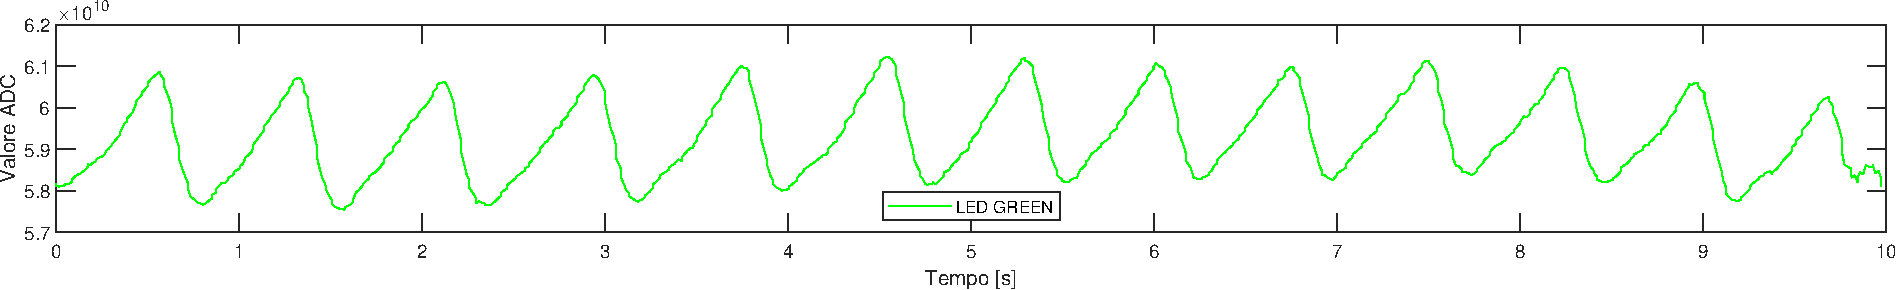
\includegraphics[width=1\linewidth]{ImageFiles/Misure Preliminari/Soggetto 2/maxm86161/polpastrello_green_moving_avg}
	\caption{Soggetto 2 - Segnali PPG acquisiti sul polpastrello del dito indice sinistro con il sensore MAXM86161.}
	\label{fig:soggetto2_MAXM86161_polpastrello}
\end{figure}

\clearpage

\paragraph{Lobo orecchio destro}
In figura \ref{fig:soggetto2_MAXM86161_lobo} sono riportati i risultati dell'acquisizione sul lobo dell'orecchio destro. Il segnale è stato filtrato con una finestra di 10 campioni per il LED verde, 30 per il LED rosso e 35 per quello infrarosso. La qualità dell'acquisizione è ancora buona, ma le ampiezze sono inferiori rispetto a quelle rilevate nell'acquisizione sul polpastrello. Questo è dovuto, come anche evidenziato precedentemente, alla difficoltà nella misura. Il segnale con ampiezza maggiore è quello ottenuto dal LED verde. Osservando il tracciato, si possono contare 11 picchi, stimando un ritmo cardiaco pari a 66 battiti al minuto.

\begin{figure}[h]
	\centering
	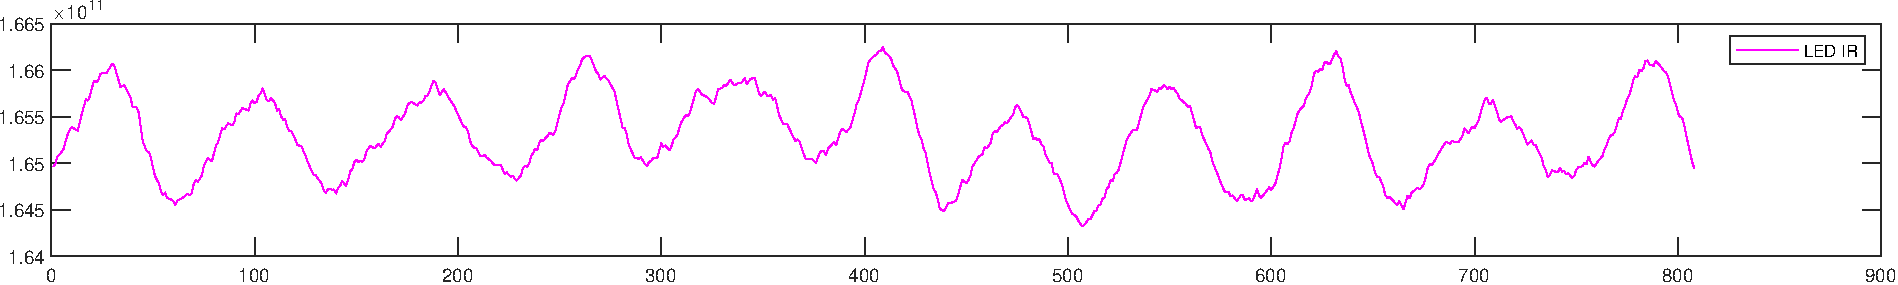
\includegraphics[width=1\linewidth]{ImageFiles/Misure Preliminari/Soggetto 2/maxm86161/lobo_ir_moving_avg}
	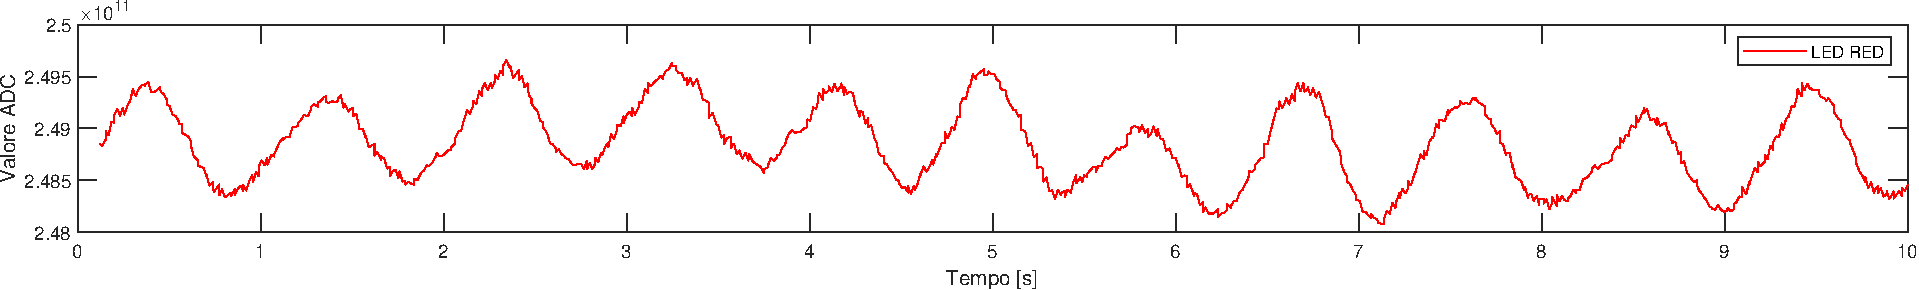
\includegraphics[width=1\linewidth]{ImageFiles/Misure Preliminari/Soggetto 2/maxm86161/lobo_red_moving_avg}
	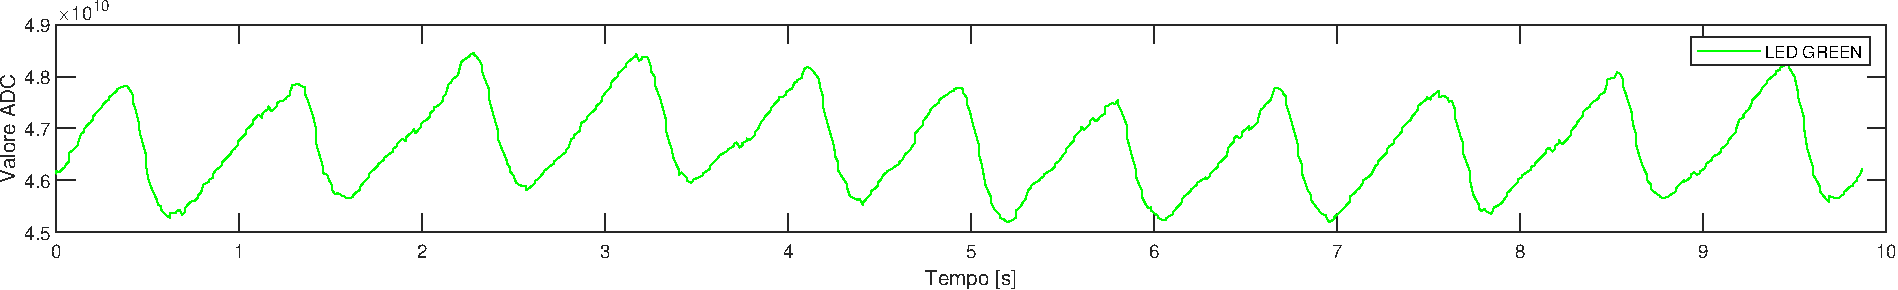
\includegraphics[width=1\linewidth]{ImageFiles/Misure Preliminari/Soggetto 2/maxm86161/lobo_green_moving_avg}
	\caption{Soggetto 2 - Segnali PPG acquisiti sul lobo dell'orecchio destro con il sensore MAXM86161.}
	\label{fig:soggetto2_MAXM86161_lobo}
\end{figure}

\clearpage

\subparagraph{Polso antero-interno}
L'acquisizione effettuata sul polso risulta invece molto rumorosa (Fig. \ref{fig:soggetto2_MAXM86161_polso}), specialmente per il segnale del LED infrarosso, mentre i segnali del LED rosso risultano discretamente buoni, sebbene alcune volte non permettono di apprezzare i picchi. La luce verde, invece, risulta avere una discreta qualità e presenta il segnale con maggiore ampiezza. Le finestre del filtro sono di 15 campioni per il LED verde e 30 per i LED rosso e infrarosso. La frequenza cardiaca stimata è di 66 battiti al minuto.

\begin{figure}[h]
	\centering
	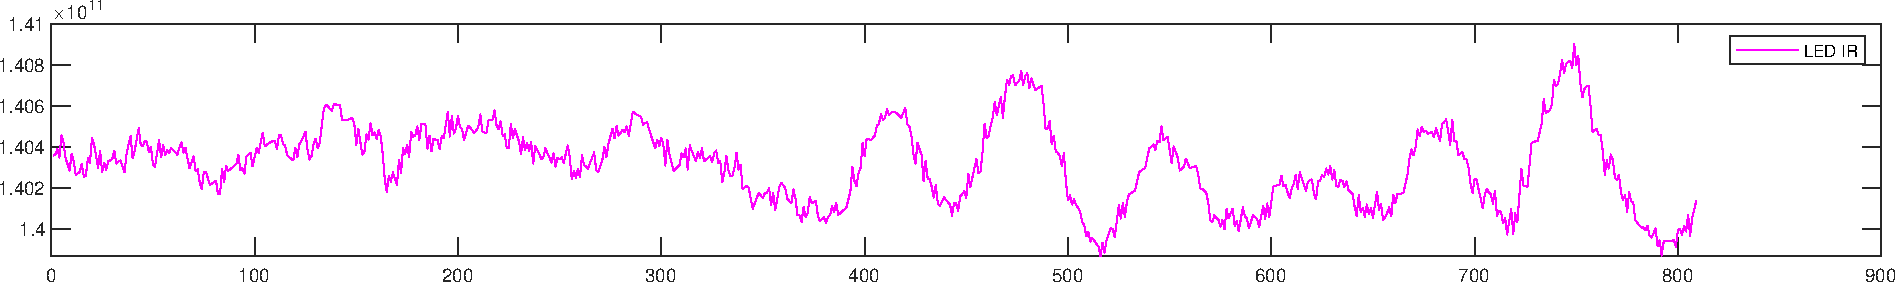
\includegraphics[width=1\linewidth]{ImageFiles/Misure Preliminari/Soggetto 2/maxm86161/polso_inferiore_ir_moving_avg}
	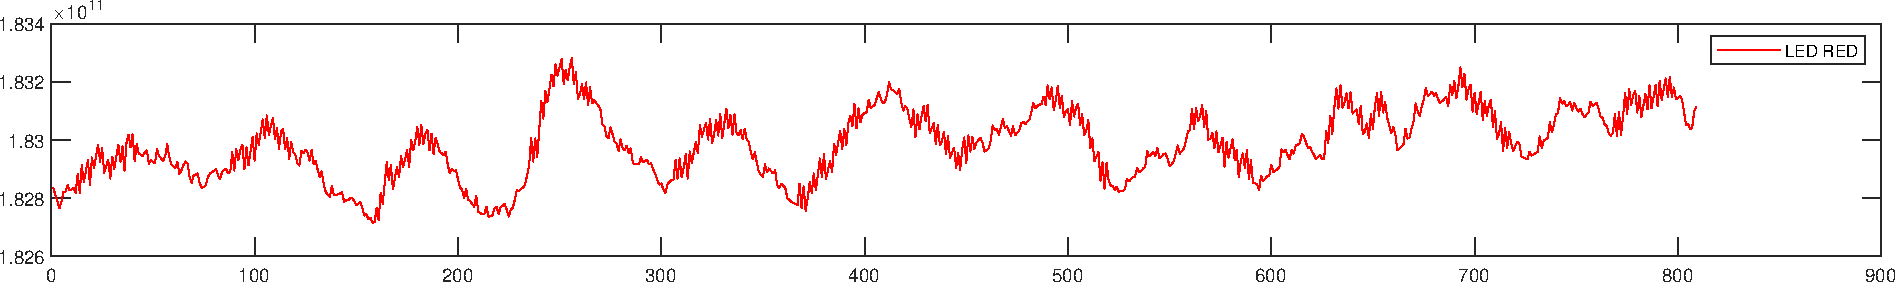
\includegraphics[width=1\linewidth]{ImageFiles/Misure Preliminari/Soggetto 2/maxm86161/polso_inferiore_red_moving_avg}
	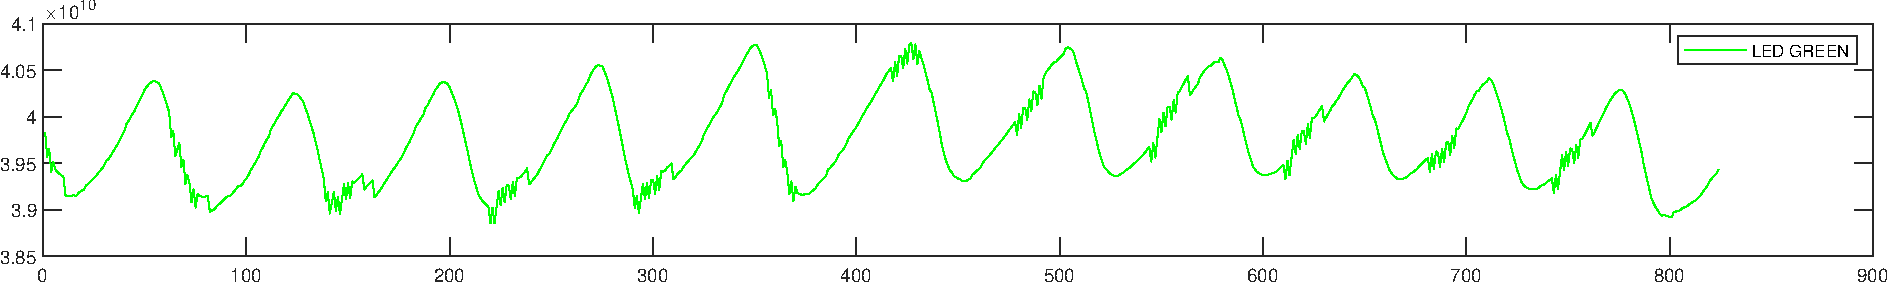
\includegraphics[width=1\linewidth]{ImageFiles/Misure Preliminari/Soggetto 2/maxm86161/polso_inferiore_green_moving_avg}
	\caption{Soggetto 2 - Segnali PPG acquisiti sul polso destro con il sensore MAXM86161.}
	\label{fig:soggetto2_MAXM86161_polso}
\end{figure}

\clearpage

\subparagraph{Fronte}
I segnali ottenuti dall'acquisizione sulla fronte, riportati in figura \ref{fig:soggetto2_MAXM86161_fronte}, sono buoni per il LED verde, mentre quelli dei LED rosso e infrarosso risultano affetti da rumore. Il filtro applicato ha una finestra di 10 campioni per il LED verde e 35 per i LED rosso e infrarosso. Il LED verde presenta il segnale a maggiore ampiezza. Dalla figura riportata, si possono individuare 11 picchi, stimando una frequenza cardiaca di 66 battiti al minuto.

\begin{figure}[h]
	\centering
	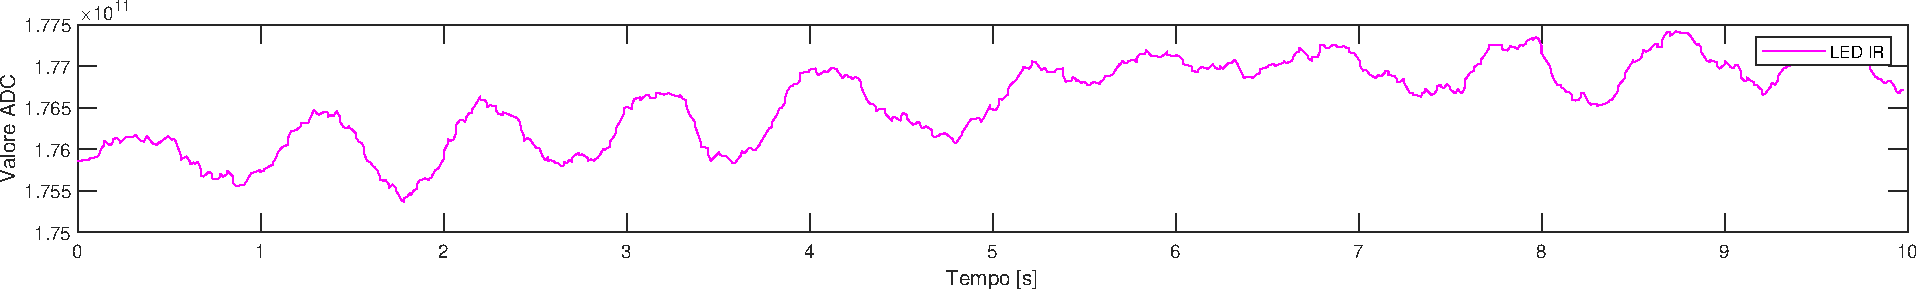
\includegraphics[width=1\linewidth]{ImageFiles/Misure Preliminari/Soggetto 2/maxm86161/fronte_ir_moving_avg}
	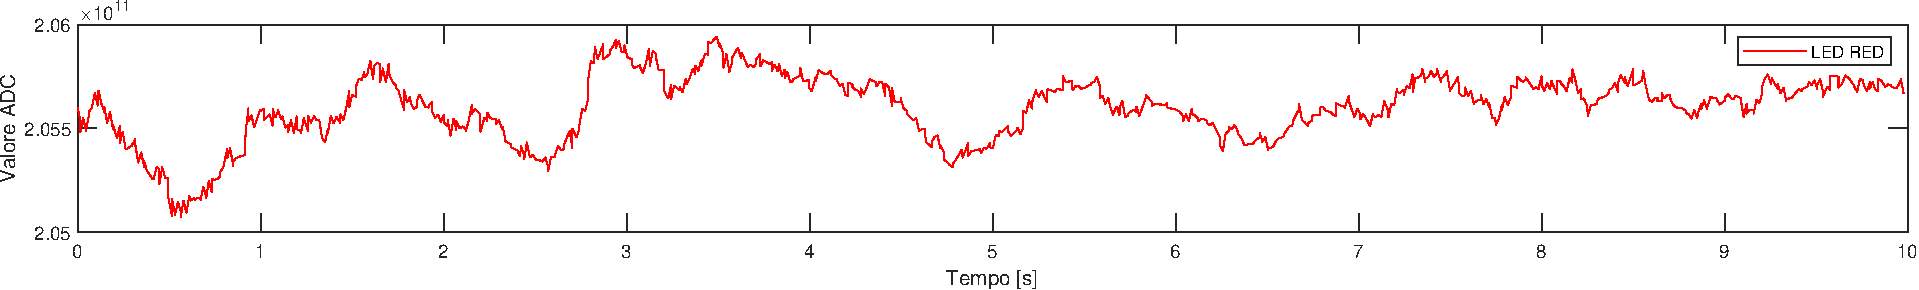
\includegraphics[width=1\linewidth]{ImageFiles/Misure Preliminari/Soggetto 2/maxm86161/fronte_red_moving_avg}
	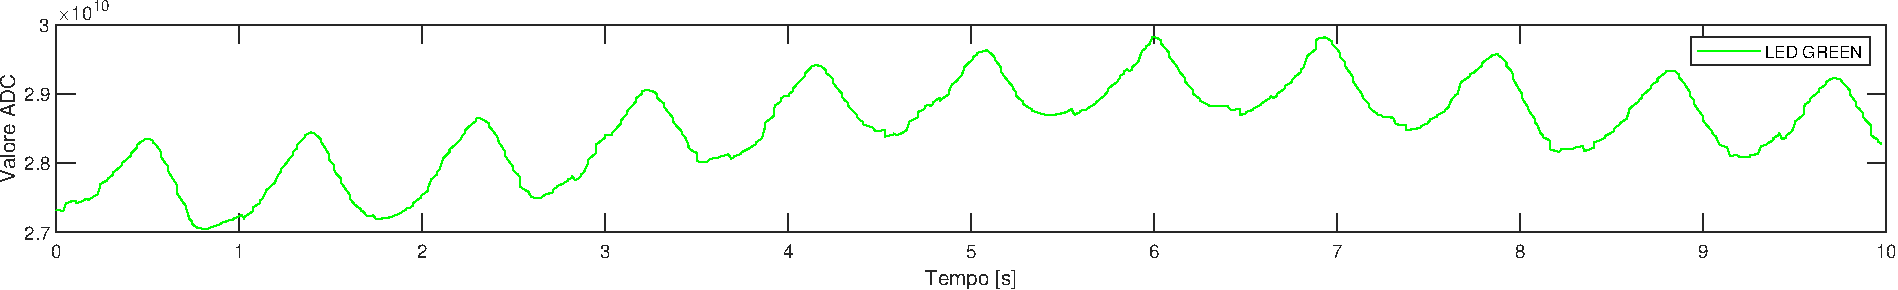
\includegraphics[width=1\linewidth]{ImageFiles/Misure Preliminari/Soggetto 2/maxm86161/fronte_green_moving_avg}
	\caption{Soggetto 2 - Segnali PPG acquisiti sulla fronte con il sensore MAXM86161.}
	\label{fig:soggetto2_MAXM86161_fronte}
\end{figure}


\clearpage